\chapter{Version Control}

\section{Software Versions}

No writer can finish a good book in one shot. A book needs to be
writen section by section and chapter by chapter. The writing is
likely reviewed and revised multiple times. If you watch a movie DVD,
you can find {\it Deleted Scenes}--- the sections that have been made
but never used in the actual movie.  Any non-trivial work needs to be
created gradually and improved over and over again before it is ready.
Developing software is no different: functionality is added
gradually. Sometimes, finished functions need to change because
customers' needs have changed, competitors have introduced new
features and modifications are needed, new regulations are announced,
or new standards are issued. All of these mean that software must be
developed in small pieces; these pieces are called {\it version}.

There is no widely accepted definition of a version, just like there
is no specific definition what should be considered as a chapter in a
book. One may consider each additional line as a new version while
another may consider a completely implemented and fully tested feature
as a version. Generally speaking, a version should be self-contained
and complete unit, like a section or a chapter in a book.  The tools
that manage versions are called {\it version control}.  When multiple
work together, version control becomes essential to ensure proper
coordination.

There are many version control systems, such {\tt CVS} (concurrent
version system) and {\tt SVN} (subversion).  This book uses {\tt git}
for version control. It is a {\it distributed} version control system,
meaning that there can be two types of {\it repositories}: One is on
each user's computer; the other is shared by all users. The advantage
of a distributed version control system will become clear after
explaining how people collaborate developing software.

The version control system {\tt git} is a set of programs managing
files.  You can run {\tt git} on your own computer. You can also set
up a {\tt git} server shared by multiple people. Alternatively, you
can use websites that offer version control functions; examples
include {\tt github.com} and {\tt bitbucket.org}.  This book uses {\tt
  github} as an example.  You can find entire books talking about {\tt
  git} as well as thousands of web postings about how to use {\tt
  github}. {\tt git} has many different functions and {\tt github}
offers many different ways to accomplish the same goals.  This book
does not intend to replace those materials.  Instead, this book
provides enough details for common needs.  Readers interested knowing
more can easily find additional documentations.

\section{\tt github}

This book chooses {\tt github} for three reasons: (1) It is widely
used.  (2) It is free for education purposes. (3) It is supported by
many tools other than the {\tt github} website.
Figure~\ref{fig:github12} shows the website of {\tt github} and the
portal for an education account.

\begin{figure}[h] \centering
 \subfigure[]
{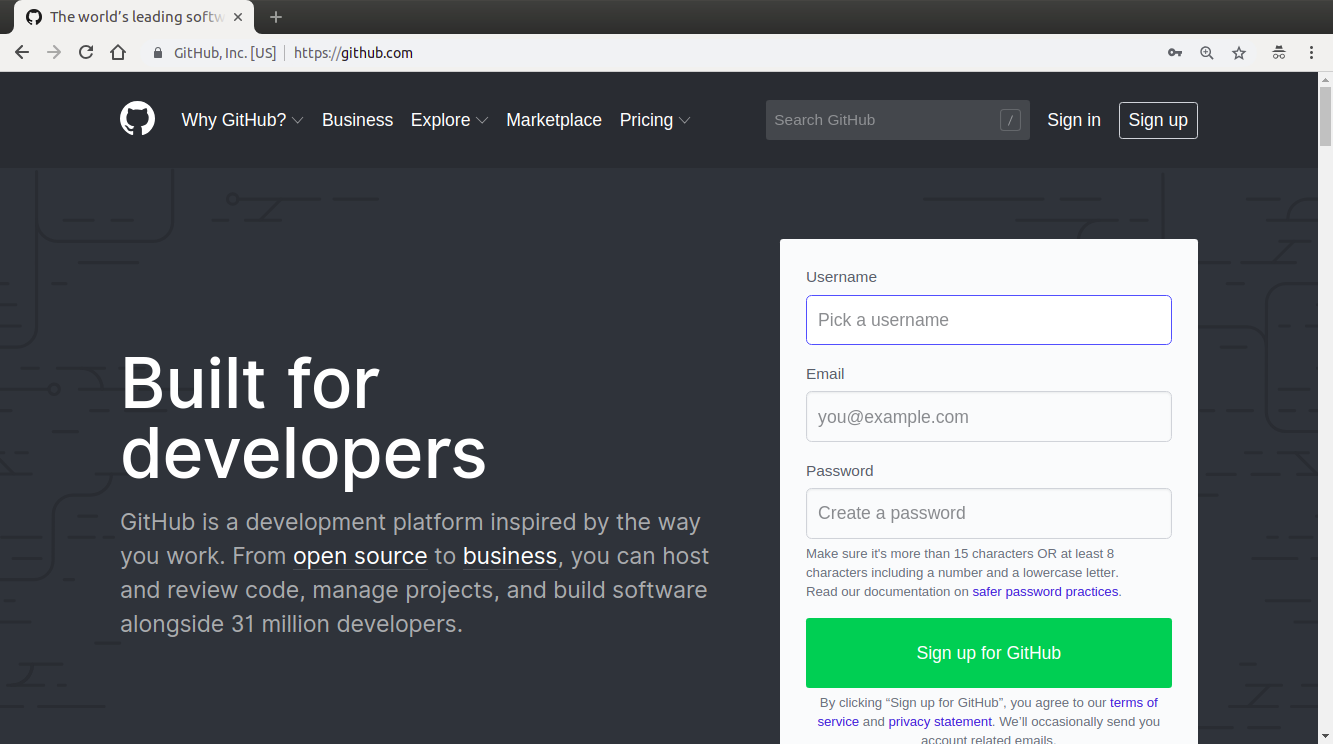
\includegraphics[width=4in]{\thischapterpath/figures/github1.png}}
  \subfigure[]
{
\includegraphics[width=4in]{\thischapterpath/figures/github2.png}}
\caption{(a) {\tt github} website. (b) Students and teachers can apply for free repositories.}
\label{fig:github12}
\end{figure}

Signing up in {\tt github} is easy, as shown in
Figure~\ref{fig:github34} (a).  After creating an account, a
repository can be created as shown in Figure~\ref{fig:github34} (b).
This website has many options: the name of the repository, whether it
is public or private, whether to initialize the repository with {\tt
  README}, etc.


\begin{figure}[h] \centering
 \subfigure[]
{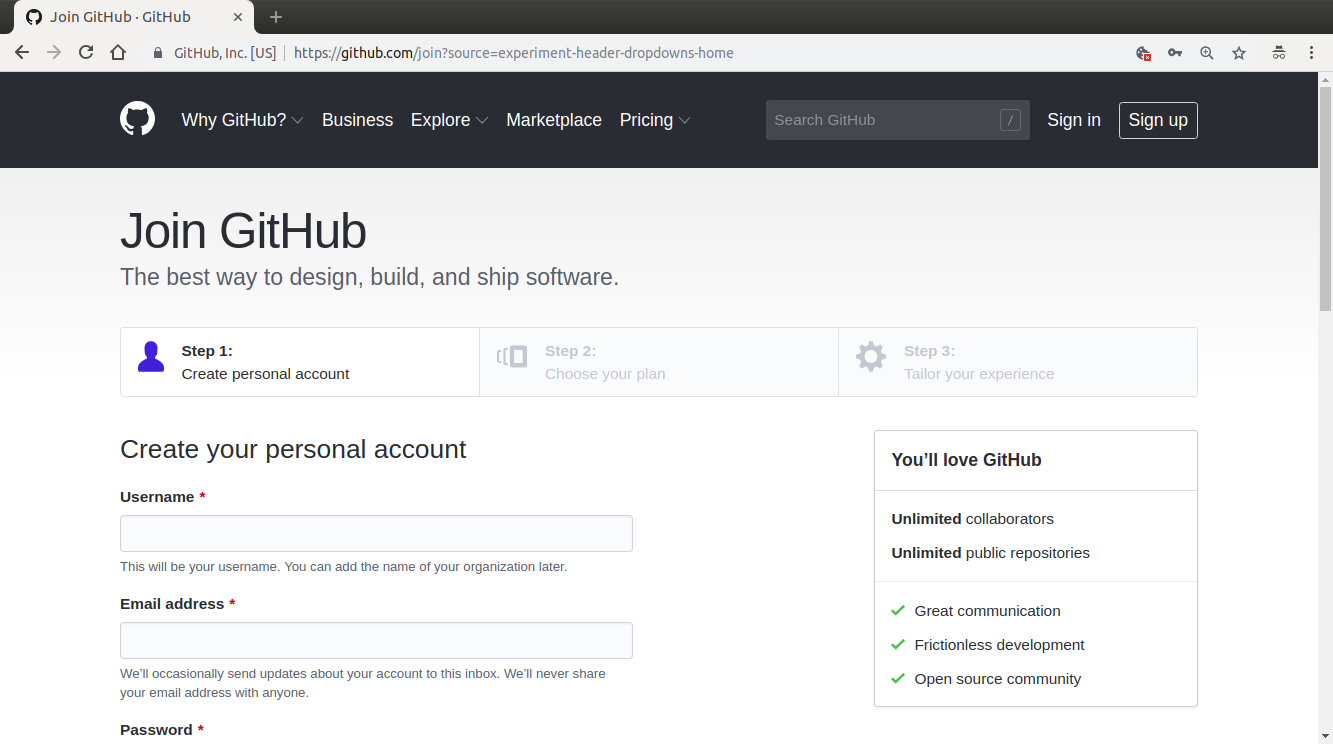
\includegraphics[width=4in]{\thischapterpath/figures/github3.png}}
  \subfigure[]
{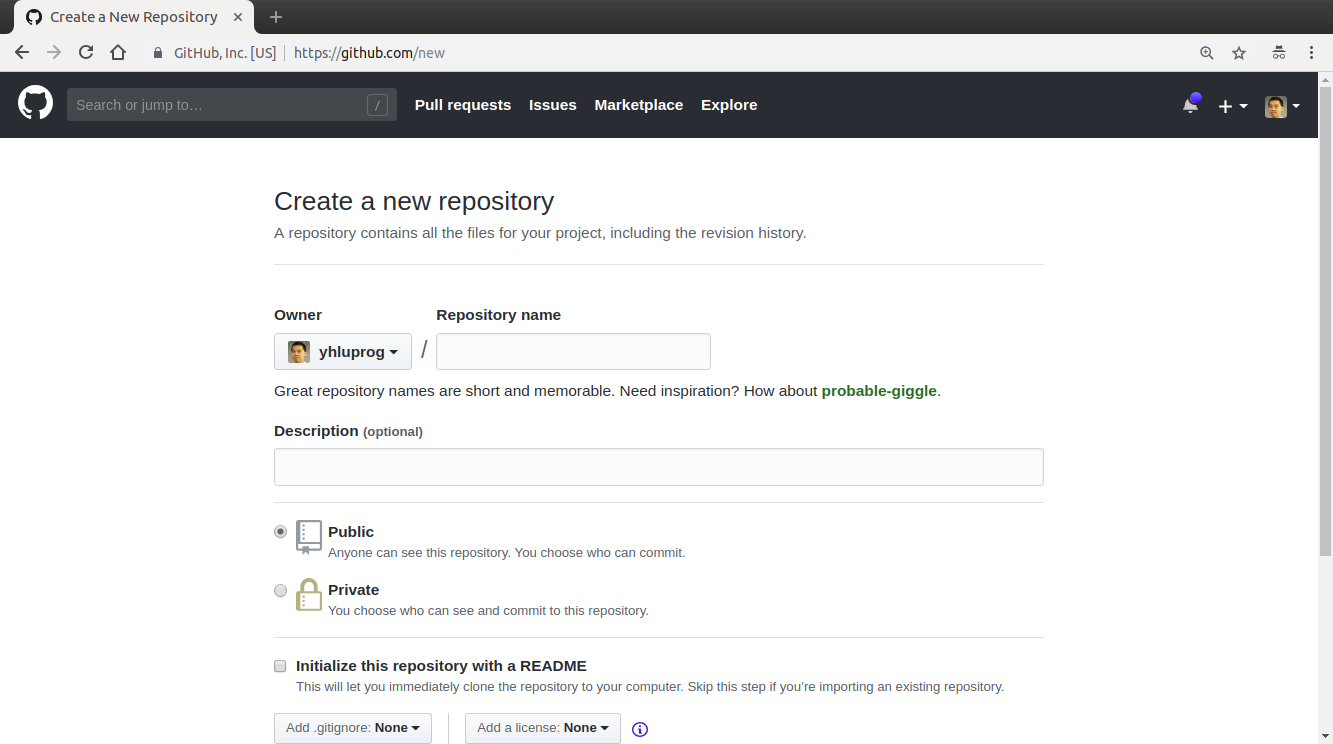
\includegraphics[width=4in]{\thischapterpath/figures/github4.png}}
\caption{(a) Create an account in {\tt github}. (b) Create a
  repository.}
\label{fig:github34}
\end{figure}

\begin{figure}[h] \centering
   \subfigure[]
{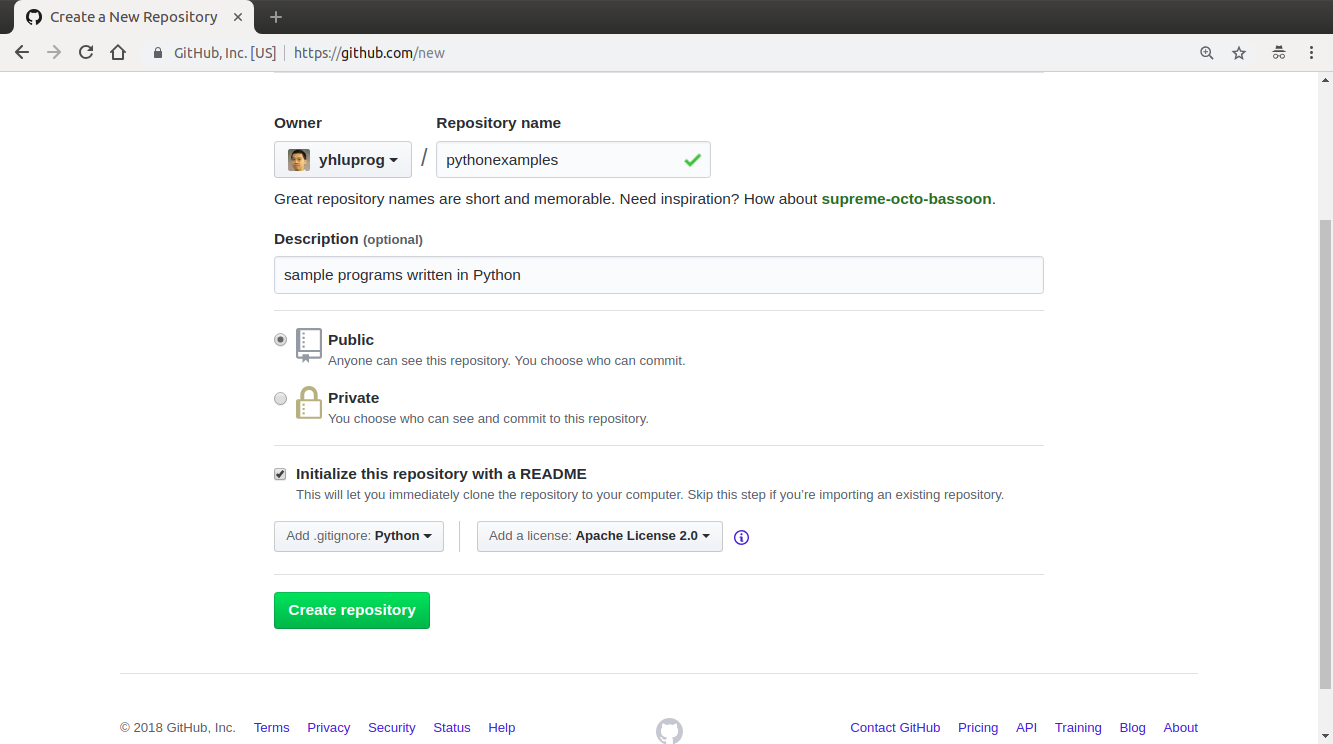
\includegraphics[width=4in]{\thischapterpath/figures/github5.png}}
   \subfigure[]
{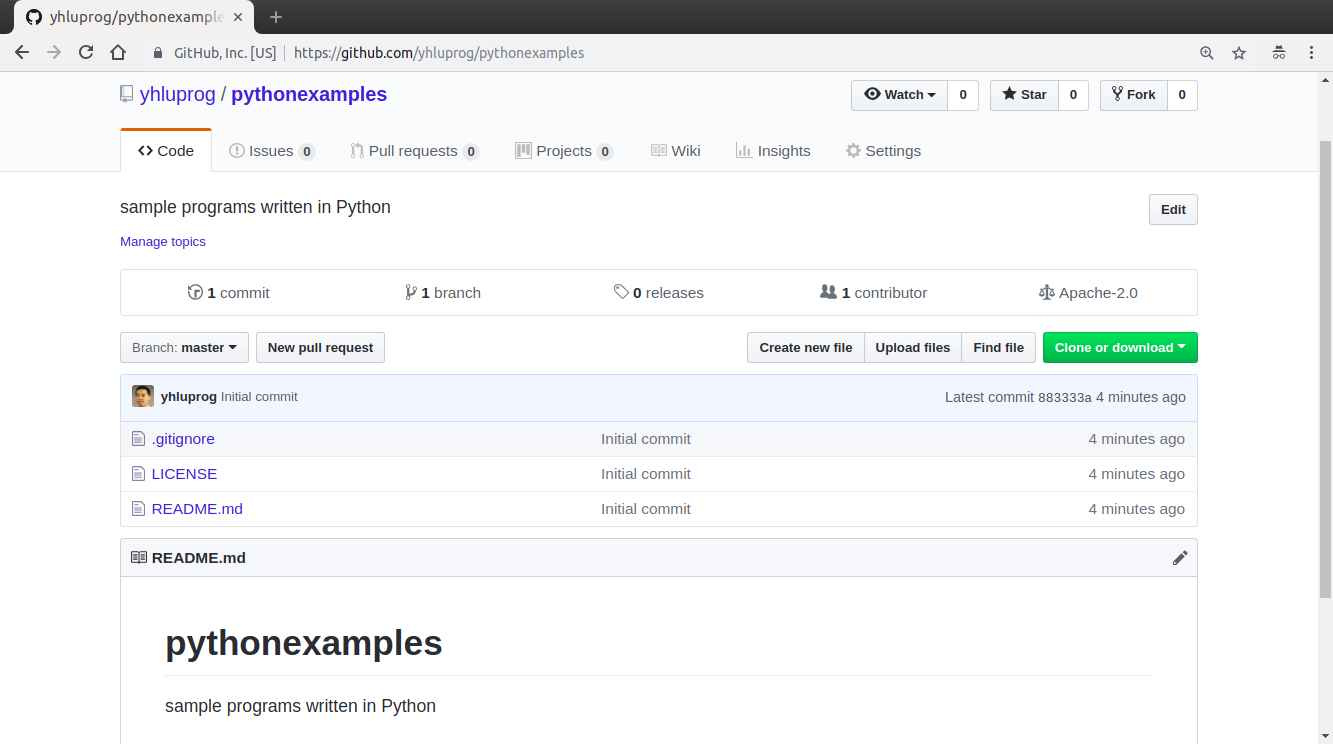
\includegraphics[width=4in]{\thischapterpath/figures/github6.png}}
\caption{(a) A new repository. (b) The repository has been created.}
\label{fig:github56}
\end{figure}

\marginnote{Is {\tt git} case sensitive? The correct answer
  is ``it is complicated''. A short answer is ``No'': you
  should treat {\tt git} as case insensitive. Do not have two
files whose names are different by cases only.}

Figure~\ref{fig:github56} (a) shows the options for creating a new repository:


\begin{itemize}
\item Repository name: pythonexamples
\item Description: sample programs written in Python
\item Public
\item Check ``Initialize this repository with a README''
\item Select ``Add .gitignore: Python''
\item Select ``Add a license: Apache License 2.0''
\end{itemize}


Figure~\ref{fig:github56} (b) shows the repository after it has been
created.  As can be seen on the website, there are many options
changing this repository.  For example, it is possible adding new
files or uploading files. It is also possible editing an file by
clicking the pen icon.

\section{Clone a Repository}

A more common way of using a repository, however, is to {\it clone} the
repository on another computer, as illustrated in Figure~\ref{fig:gitclone}.

\begin{figure}[h] \centering
{
\includegraphics[width=3in]{\thischapterpath/figures/gitclone.png}}
\caption{Using {\tt git clone} command creates a repository on another computer.}
\label{fig:gitclone}
\end{figure}

To clone a repository, it is necessary knowing the {\it path} in {\tt
  github}.  Figure~\ref{fig:github7} shows the path of the repository.

\begin{figure}[h] \centering
{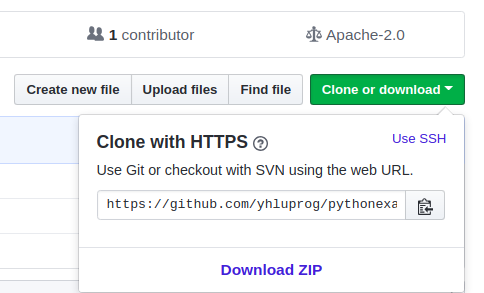
\includegraphics[width=3in]{\thischapterpath/figures/github7.png}}
\caption{Cloning a repository may use HTTPS or SSH.}
\label{fig:github7}
\end{figure}


\clearpage

To clone the repository, starts a {\it Terminal} in Linux
and type the {\tt git clone} command. In the following
example, {\tt \$} is the {\it command prompt} for the Terminal.

\vspace{0.2in}

\noindent
\begin{tabular}{|p{5in}|}\hline
\begin{verbatim}
$ git clone https://github.com/yhluprog/pythonexamples.git
\end{verbatim}
\\ \hline
\end{tabular}
\vspace{0.2in}

The command clones the repository and the following message is shown:

\vspace{0.2in}

\noindent
\begin{tabular}{|p{5in}|}\hline
\begin{verbatim}
Cloning into 'pythonexamples'...
remote: Enumerating objects: 5, done.
remote: Counting objects: 100% (5/5), done.
remote: Compressing objects: 100% (5/5), done.
remote: Total 5 (delta 0), reused 0 (delta 0), pack-reused 0
Unpacking objects: 100% (5/5), done.
Checking connectivity... done.
\end{verbatim}
\\ \hline
\end{tabular}
\vspace{0.2in}

After cloning the repository, a directory (also called folder) with
the name {\tt pythonexamples} is created.  This can be shown
using the {\tt ls} command:

\vspace{0.2in}

\noindent
\begin{tabular}{|p{5in}|}\hline
\begin{verbatim}
$ ls
pythonexamples/
\end{verbatim}
\\ \hline
\end{tabular}
\vspace{0.2in}

Inside this directory, there are already two files: {\tt
  LICENSE} and {\tt README.md}. The is a hidden file {\tt .gitignore}.
It is hidden because it starts with {\tt .} and is not shown by the
{\tt ls} command. To show a hidden file, it is necessary using the
{\tt ls -a} command. Additionally, a hidden directory (ending with
{\tt /}) called {\tt .git} is also shown.

\vspace{0.2in}

\noindent
\begin{tabular}{|p{5in}|}\hline
\begin{verbatim}
$ cd pythonexamples/
$ ls -a
./  ../  .git/	.gitignore  LICENSE  README.md
\end{verbatim}
\\ \hline
\end{tabular}
\vspace{0.2in}

Enter the directory using the {\tt cd} command
and use the {\tt ls} command to see the files and directories.

\vspace{0.2in}

\noindent
\begin{tabular}{|p{5in}|}\hline
\begin{verbatim}
$ cd .git
$ ls
branches/  config  description	HEAD  hooks/  index  
info/  logs/  objects/  packed-refs  refs/
\end{verbatim}
\\ \hline
\end{tabular}
\vspace{0.2in}


Among them, {\tt config} stores the information about
the remote repository.  The {\tt more} command can show
the content of the file:

\vspace{0.2in}

\noindent
\begin{tabular}{|p{5in}|}\hline
\begin{verbatim}
$ more config
[core]
	repositoryformatversion = 0
	filemode = true
	bare = false
	logallrefupdates = true
[remote "origin"]
	url = https://github.com/yhluprog/pythonexamples.git
	fetch = +refs/heads/*:refs/remotes/origin/*
[branch "master"]
	remote = origin
	merge = refs/heads/master
\end{verbatim}
\\ \hline
\end{tabular}
\vspace{0.2in}

The line starting with {\tt url} is the path used in {\tt git clone}.
The concept of {\it branch} will be explained later in this chapter.

\section{Commit and Push}

\marginnote{Modifying {\tt LICENSE} is not recommended.}

There are many different methods modifying a repository.  The first
method modifies an existing file.  Use a text editor and add the
following line to {\tt README.md}:

\begin{verbatim}
This repository demonstrates how to use commit, push, and branch.
\end{verbatim}

After adding this line, use the {\tt git commit} command to show which file
has been changed:

\vspace{0.2in}

\noindent
\begin{tabular}{|p{5in}|}\hline
\begin{verbatim}
$ git commit
On branch master
Your branch is up-to-date with 'origin/master'.
Changes not staged for commit:
	modified:   README.md
\end{verbatim}
\\ \hline
\end{tabular}
\vspace{0.2in}

What does this mean? It says a file {\tt README.md} has been changed
but it has not been committed. The next question is the difference
between changes and commit.  Modifications are often reviewed and
revised multiple times; these changes are transient and do not need to
be recorded in the repository.  When the modifications are
satisfactory, the file is ready to ``take a snapshot'' by creating a
new version.  The command to take a snapshot is {\tt git commit}.

The earlier {\tt git commit} shows the candidate(s) for commit.  A
candidate can be a files that has been modified ({\tt README.md} in
this example).  This command has not committed any changes yet and has
not created a new version.
